\documentclass[graphics]{beamer}

\usepackage{graphicx}
\usepackage{verbatim}
\usepackage{wrapfig}
\useoutertheme{shadow}
%\usecolortheme{orchid}
\usecolortheme{seahorse}


% math commands
\newcommand{\be}{\begin{eqnarray}}
\newcommand{\ee}{\end{eqnarray}}
\newcommand{\beq}{\begin{equation}}
\newcommand{\eeq}{\end{equation}}
\def\simless{\mathbin{\lower 3pt\hbox
      {$\rlap{\raise 5pt\hbox{$\char'074$}}\mathchar"7218$}}}
\def\simgreat{\mathbin{\lower 3pt\hbox
      {$\rlap{\raise 5pt\hbox{$\char'076$}}\mathchar"7218$}}} %> or of order

% variables

\def\toonscale{0.45}
\def\mboxy#1{\mbox{\small #1}}


\begin{comment}
\AtBeginSection[]{
  \frame{
    \frametitle{Outline}
    \tableofcontents[currentsection]
  }
}
\end{comment}

\title{Cosmic Neutrinos
}
\subtitle{}
\author[U. Pen]{\textcolor{green}{H. Zhu,Y. Yu,
 H. Yu, J.D. Emberson, D. Inman, Q. Pan, X.Wang,
and many more}
\\[8mm] 
}
\date{October 25, 2017}


\begin{document}

\frame{
\begin{picture}(320,250)
\put(-50,-130){
\includegraphics[width=5.5in]{Figures/delta_nu_sim.pdf}}
\end{picture}
\vspace{-3in}
\titlepage
}

%\section*{Introduction}
\section{Cosmological Neutrinos}

\begin{comment}
  \subsection{Outline}

  \frame{
    \frametitle{Outline}
    \tableofcontents
  }
\end{comment}

  \frame{
\vspace{-0.5in}
    \frametitle{Neutrinos}
    \begin{itemize}
    \item 3 neutrino generations: $\nu_e,\, \nu_\mu,\, \nu_\tau$
    \item quantum superposition of 3 mass states
    \item Majorana vs Dirac
    \item normal or inverted mass hierarchy?
    \item link to matter-anti-matter asymmetry?
    \item link to LIGO, GRB?
    \end{itemize}
  }


\frame{
\frametitle{Neutrino Basics}
\begin{itemize}
\item weak interaction $\beta$ decay lepton number conservation: $n\longrightarrow
  p+e^-+\bar{\nu}_e$
\item all interactions are left handed
\item propagates in mass eigenstate
\item phases mix in propagation, changes measured flavour
\item 2015 Nobel Prize to Kajita and McDonald
\item important experiments in China: Daya Bay, JUNO
\end{itemize}
}

  \frame{
    \frametitle{Oscillations}
\includegraphics[width=3.5in]{Figures/neutrino_oscillations.png}  Vogel+2014
}


\frame{
    \frametitle{Cosmic Neutrinos}
    \begin{itemize}
    \item left hand $\nu$'s interaction at $T \gg $MeV, affects
      nucleosynthesis      
    \item If Majorana: anti particle and handedness degenerate
    \item if Dirac: right helical $\nu$ distinct from left $\bar{\nu}$,
      twice as many particles
    \item standard model annihilation heats left $\nu$: twice as hot
    \item average left $\nu$ density today 112 $\nu$/cm$^3$
   \end{itemize}
  }


  \frame{
 \frametitle{Cosmic Neutrino Background}
\begin{itemize}
    \item gravitational clustering poorly understood
    \item minimum high mass 0.05 eV: $\Omega_\nu \sim 10^{-3} \ll \Omega_b$
    \item most massive neutrino non-relativistic today, affects LSS
    \item cosmological probes: how to disentangle such a small
          effect
    \end{itemize}
  }

  \frame{
    \frametitle{Neutrino messengers}
    \begin{itemize}
        \item CDM and baryonic particles in milky way come from within 1 Mpc
          primordially: very local
        \item neutrinos come from 100 Mpc.
    \end{itemize}
}


  \frame{
    \frametitle{Non-linear dynamics}
    \begin{itemize}
        \item $\nu$'s moving in non-linear CDM potential
        \item initially high thermal dispersion: Poisson noise
        \item sample phase space distribution
        \item measure gravitational back reaction
        \item supercomputer to the rescue!
    \end{itemize}
\vspace{-0.1in}\hspace{.3in}
\includegraphics[width=2.2in]{Figures/th2photo.jpg}
}
  \frame{
    \frametitle{Movie}
    {\tt http://cita.utoronto.ca/\~\,haoran/thnu/movie.html}
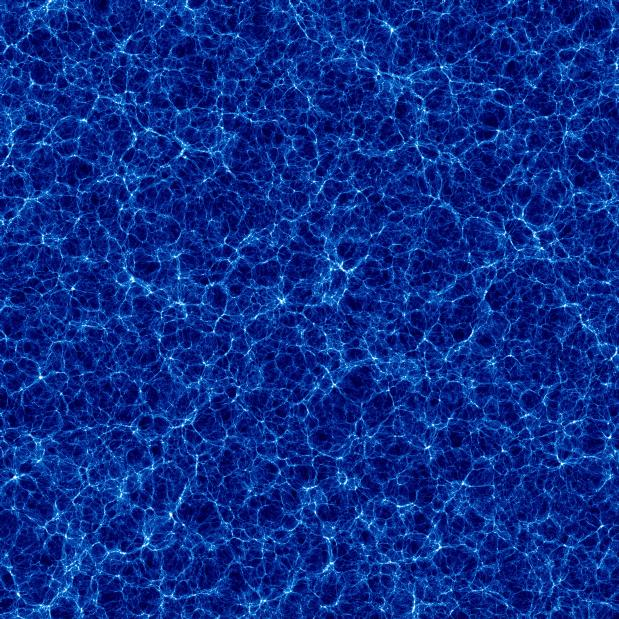
\includegraphics[width=4.2in]{Figures/thnucdmlowres.jpg}
}
  \frame{
    \frametitle{Differential clustering}
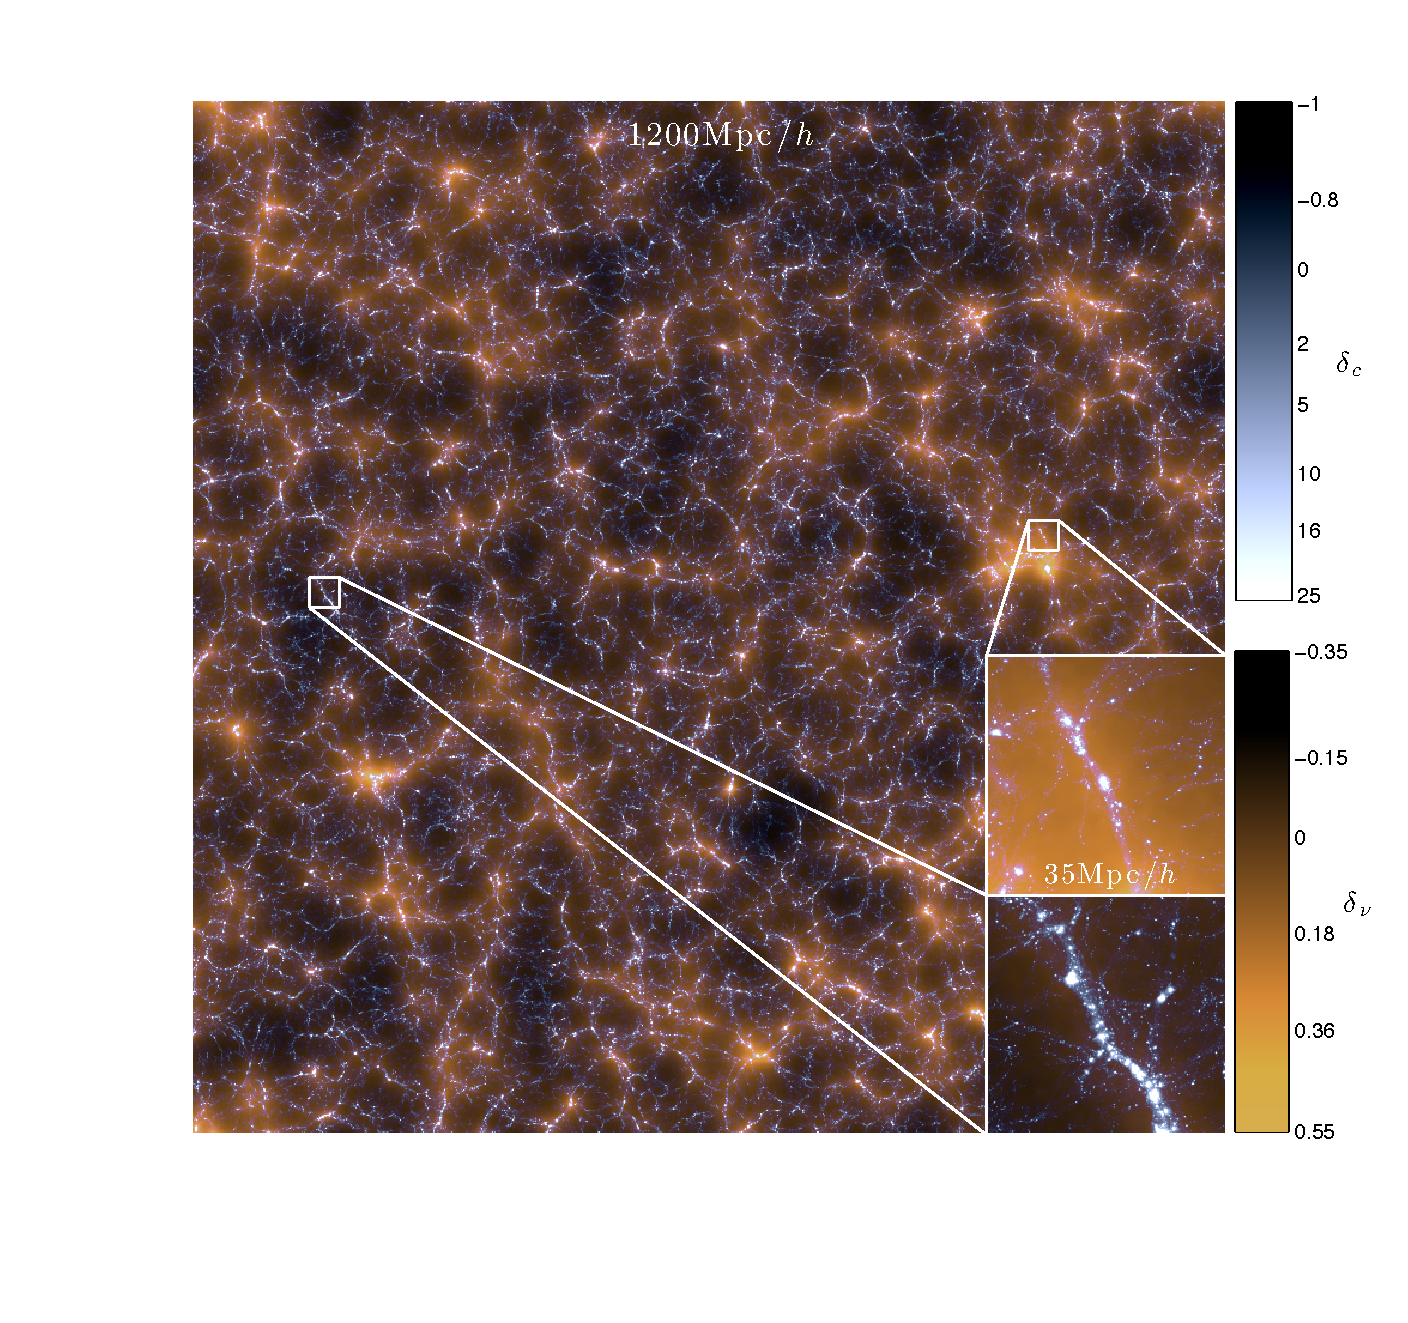
\includegraphics[width=3.5in]{Figures/cnudiff.pdf}Yu++ 2017
}
  \frame{
    \frametitle{$\nu$ -bias}
\vspace{-1.0in}
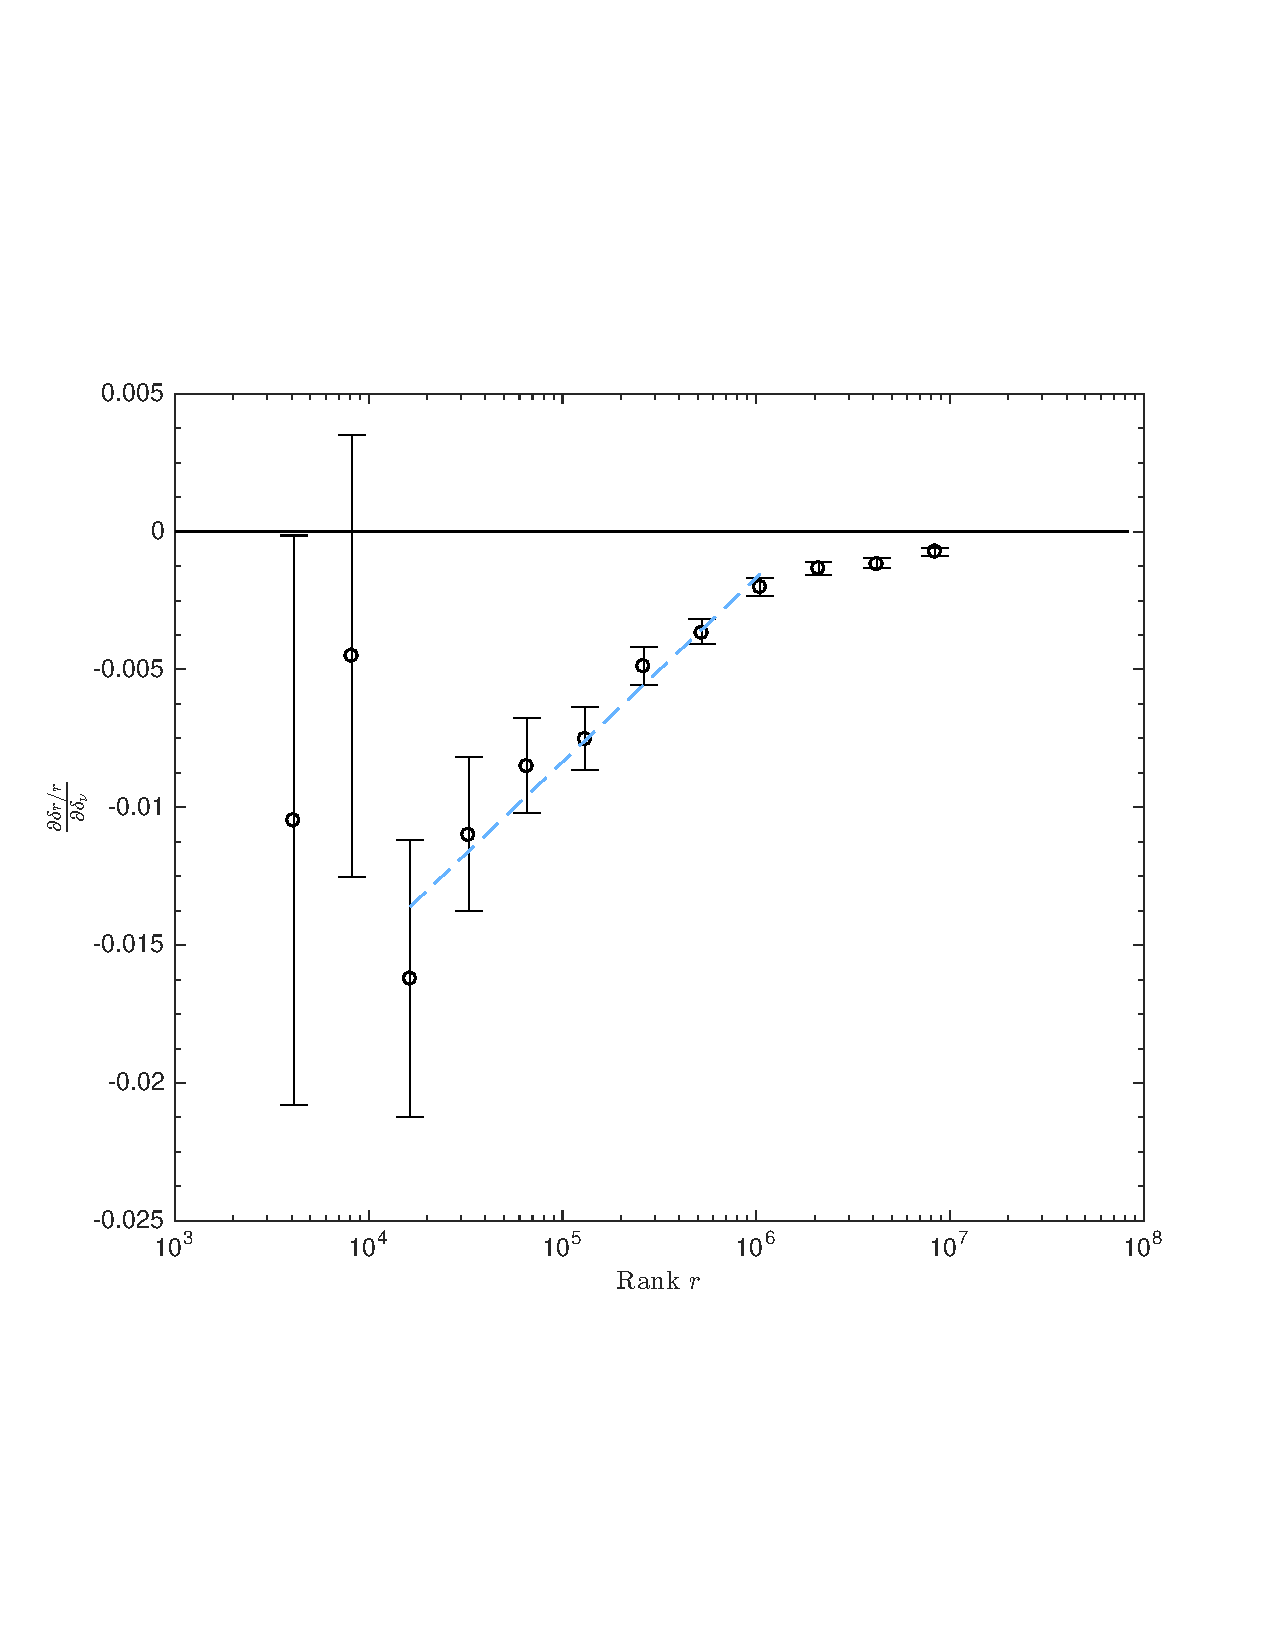
\includegraphics[width=4.0in]{Figures/slope_fit} 
}



\frame{
%\vspace{-0.5in}
    \frametitle{LIGO}
    \begin{itemize}
      \item surprising detection of 30 M$_\cdot$ binaries
      \item Nobel Prize 2017: Barish, Thorne, Weiss
      \item association with GRB
     \end{itemize}
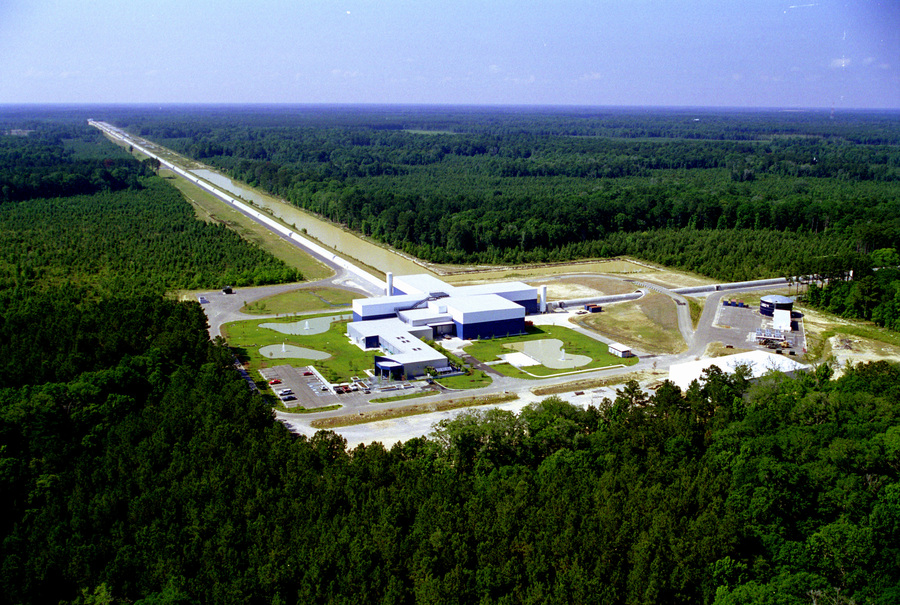
\includegraphics[width=3.0in]{Figures/ligo-livingston-aerial-02.jpg}
  }

\frame{
%vspace{-0.5in}
    \frametitle{Primordial Black Holes}
    \begin{itemize}
      \item would form from 5-$\sigma$ peaks (Bird++ 2016) at $T\sim$ 100
        MeV (Turok+ULP 2016)
      \item significant neutrino damping, possible pulsar timing signature
     \end{itemize}
 \includegraphics[width=3.0in]{Figures/whitedata_strain_SNR_qscan_v11Vhigh.jpg}
 }
\frame{
    \frametitle{image}
%\hspace{-1.1in}
\includegraphics[width=4.5in]{Figures/LIGO_blackhole.jpg}
 }



\frame{
\vspace{-0.5in}
    \frametitle{Matter asymmetry}
    \begin{itemize}
      \item why is more matter than anti-matter in universe?
      \item standard electroweak model violated baryon number through
        anomaly, B+L violated, B-L conserved
      \item Sacharov criteria: 1. B violation, 2. C, CP violation,
        3. non-thermal
      \item either before 200 GeV, perhaps L violation in neutrino sector,
        then converted to B through electro-weak anomaly
      \item during or after 200 GeV: phase transition
     \end{itemize}
  }

\frame{
\vspace{-0.5in}
    \frametitle{Electro-weak domain walls}
    \begin{itemize}
      \item generic in MSSM
      \item global symmetry in Higgs field, domain walls form at 200 GeV
      \item QCD instantons break symmetry, walls annihilate at 100 MeV
      \item 2000x scale factor for catalytic baryogenesis
      \item weakly inhomegeneous BBN
     \end{itemize}
  }

\frame{
\vspace{-0.5in}
    \frametitle{Catalytic explosions}
    \begin{itemize}
      \item Electroweak nucleation runaway for densities $>$ (100
        MeV)$^4$ (QCD scale)
      \item satisfied by neutron stars
      \item instabilities (Chandrasekar?) may lead to explosion
      \item Higgs vacuum decays to neutrinos
      \item signature in ICECUBE
     \end{itemize}
  }

\frame{
%\vspace{-0.5in}
    \frametitle{GW170817}
    \begin{itemize}
      \item GRB 170817A: neutron star merger, @40 Mpc
      \item unusual GRB signature, probably kilonova breakout, low
        lorentz factor
      \item no ICECUBE neutrinos detected
     \end{itemize}
\includegraphics[width=2.9in]{Figures/GW_Versus_Matter_STILL__CREDIT__Karan_Jani_Georgia_Tech.jpg}
  }

\frame{
\vspace{-0.5in}
    \frametitle{Conclusions}
    \begin{itemize}
      \item Cosmos filled with neutrinos
      \item challenging detection
      \item may contain key to several cosmic mysteries
      \item baryon asymmetry?
     \end{itemize}
  }


\end{document}
